\documentclass[letter,11pt]{article}

\usepackage[margin=1in]{geometry}
\usepackage[utf8]{inputenc}
\usepackage{color}
\usepackage{xcolor}
\usepackage{amsmath}
\usepackage{amssymb}
\usepackage{amsthm}
\usepackage{hyperref}
\usepackage{graphicx}
\usepackage{tikz}
\usepackage{caption}
\usepackage{float}
\usetikzlibrary{positioning,arrows.meta}




\begin{document}

\noindent\rule[2mm]{\textwidth}{1.5mm}
\noindent
\begin{minipage}{.3\textwidth}
  \vspace{-3mm}
  {\Huge\bf HW 3}
\end{minipage}\hfill\begin{minipage}{.5\textwidth}
\begin{flushright}
  {\bf Intro Algorithms EN.601.433 \\
  Fall 2023 \\
  Due: Friday 10/13/2023 at 11:59 PM}%
\vspace{3mm}
\end{flushright}
\end{minipage}
\noindent\rule{\textwidth}{1.5mm}

\section*{Instructions}

\begin{itemize}
\item This homework is worth 10\% of your final grade.

\item This homework is due Friday 10/13/2023 at 11:59 PM on
  Gradescope.  Solutions will be posted on Canvas at midnight.  No late homework will be accepted.  To access Gradescope, click the Gradescope link on Canvas.

\item You are \textbf{required} to type your homework.  We will
  provide the \LaTeX{} source code to the homework assignments, which you may
  optionally use as a template.  If you install \LaTeX{} on your computer, you can
  generate a PDF of
  your homework by running the command: \\
  \\
  \texttt{latexmk~-pdf~my-homework.tex} \\
  \\
  Alternately, you can use \url{https://www.overleaf.com/edu/jhu} as a web based
  \LaTeX~editor.

\item You can collaborate with one other person.
    Collaboration should happen through verbal communication, scratch paper,
    whiteboards, etc.  You are \textbf{not} allowed to copy homework
    solutions from another student.  All students are required to submit their
    own write-up.

\item You are \textbf{not} allowed to use any website to find solutions to these problems.

\item Do not write your name on your homework. Instead, write your Johns Hopkins Student ID.  This will allow us to grade your homework anonymously.

\item For questions that require you to write an algorithm out, you can either use pseudo-code or English description.

\item Make sure that you correctly assign which page a problem is located on when uploading to Gradescope.

\item For problems that require graphs or diagrams, you are allowed to include an image of a drawing instead of typesetting the graph.\footnote{If you are using LaTeX, you can follow the instructions here \url{https://www.overleaf.com/learn/latex/Inserting_Images} to embed an image in LaTeX.}
\end{itemize}


\newpage
%%%%%%%%%%%%%%%%%%%%%%%%%%%%%%%%%%%%%%%%%%%%%%%%%%%%%%%%%%%%%%%%%%%%%%%%%%%%%%%%%%%%%%%%%%%%%%%%%%%%
%  _    ___          __  _____           _     _
% | |  | \ \        / / |  __ \         | |   | |
% | |__| |\ \  /\  / /  | |__) | __ ___ | |__ | | ___ _ __ ___  ___
% |  __  | \ \/  \/ /   |  ___/ '__/ _ \| '_ \| |/ _ \ '_ ` _ \/ __|
% | |  | |  \  /\  /    | |   | | | (_) | |_) | |  __/ | | | | \__ \
% |_|  |_|   \/  \/     |_|   |_|  \___/|_.__/|_|\___|_| |_| |_|___/
%%%%%%%%%%%%%%%%%%%%%%%%%%%%%%%%%%%%%%%%%%%%%%%%%%%%%%%%%%%%%%%%%%%%%%%%%%%%%%%%%%%%%%%%%%%%%%%%%%%%


\section{Scheduling Computation (6 points)}


The wildly popular Spanish-language search engine El Goog needs to do a serious amount of computation every time it recompile its index. Fortunately, the company has at its disposal a single large supercomputer, together with an essentially unlimited supply of high-end PCs.

They've broken the overall computation into n distinct jobs, labeled $J_1$, $J_2$, \dots, $J_n$, which can be performed completely independently of one another. Each job consists of two stages: first it needs to be pre-processed on the supercomputer, and then it needs to be finished on one of the PCs. Let’s say that job $J_i$ needs $p_i$ seconds of time on the supercomputer, followed by $f_i$ seconds of time on a PC.

Since there are at least $n$ PCs available on the premises, the finishing of the jobs can be performed fully in parallel—all the jobs can be processed at the same time. However, the supercomputer can only work on a single job at a time, so the system managers need to work out an order in which to feed the jobs to the supercomputer. As soon as the first job in order is done on the supercomputer, it can be handed off to a PC for finishing; at that point in time a second job can be fed to the supercomputer; when the second job is done on the supercomputer, it can proceed to a PC regardless of whether or not the first job is done (since the PCs work in parallel); and so on.

Let's say that a schedule is an ordering of the jobs for the supercomputer, and the completion time of the schedule is the earliest time at which all jobs will have finished processing on the PCs. This is an important quantity to minimize, since it determines how rapidly El Goog can generate a new index.\\


Give a polynomial-time algorithm that finds a schedule with as small a completion time as possible. You should also prove that your algorithm results in an optimal solution, and it needs to be a formal proof.

\subsection{Solution: Algorithm}

No matter what order the jobs are scheduled in, we must wait for every job to pre-process before we complete the jobs. Therefore, no matter which job is scheduled last, it must wait for a combined time of the sum of every previous job's pre-processing time before it can finalize. For the entire runtime, let's say that we have $i$ jobs. Then, job $j_i$ can only be started when we have finished pre-processing every job before it, at time $T = \sum^{i}_{n=1} p_i$. Since the time it takes for the supercomputer to start on the last job $j_i$ is fixed, we must try to minimize the amount of time it takes to finalize the last job, or $f_i$. \\

Therefore, we can use a sorting algorithm to order the jobs with the longest finalizing time first, and the shortest finalizing time last. We can use a simple efficient sorting algorithm like quicksort, which runs in $O(n\log{}n)$.  Therefore, our algorithm is as follows. \\

Given a schedule of jobs, we can sort them in decreasing order by completion time $f_i$ using quicksort. \\

Then, run them through the supercomputer, wait for the job to finish pre-processing, and finalize them in parallel in the conditions given above.\\

\subsection{Solution: Formal Proof}

Let's first consider the time of completion $c_i$ for each job, where $c_j = \sum_{i=1}^{n}{p_i} + f_j$. As calculated, the pre-processing time of completion for each job depend on the jobs that pre-process before them. \\

Suppose that in the optimal schedule, the jobs run in an order where job $k$ has the longest completion time $c_k$, and is not first job in the sequence. Also consider the shortest job, denoted as job $j$. Consider a schedule containing only these jobs. In the "optimal" schedule, if the completion time of the job with the longer finishing time is the job with the higher completion time, then our algorithm improves on it by reducing the completion time of the job with the longer finishing time. Since $\sum_{i=1}^{n}{p_i} + f_j < \sum_{i=1}^{n}{p_i} + f_k$, if the change results in the job with the shorter finishing time becoming the job with the higher completion time, it is still better than the optimal schedule.\\

We can apply this concept to a schedule with any number of jobs, and we can do the same comparison with any pair of jobs in said schedule, repeating until we cannot improve the runtime any more. With this, we have sorted the jobs in order of decreasing finishing times, which is what our algorithm does, providing an optimal schedule.

\subsection{Solution: Time Complexity}

Our algorithm runs on a polynomial time complexity. Quicksort is $O(n\log{}n)$, and the actual running of the jobs (feeding them into the supercomputer and then the PCs) takes $O(2n) = O(n)$. This means the entire runtime of the algorithm with the running of the schedule is $O(n\log{}n) + O(n) = O(n\log{}n)$, which is polynomial runtime.





\section{CluNet Needs To Get A Clue (6 points)}

A group of network designers at the communications company CluNet find themselves facing the following problem. They have a connected graph $G =(V,E)$, in which the nodes represent sites that want to communicate. Each edge $e$ is a communication link, with a given available bandwidth $b_e$.

For each pair of nodes $u$, $v\in V$, they want to select a single $u-v$ path $P$ on which this pair will communicate.  The bottleneck rate $b_{(P)}$ of this path $P$ is the minimum bandwidth of any edge it contains; that is, $b_{(P)}=min_{e\in P} b_e$. The best achievable bottleneck rate for the pair $(u,v)$ in $G$ is simply the maximum, over all $u-v$ paths $P$ in $G$, of the value $b_{(P)}$.

It's getting to be very complicated to keep track of a path for each pair of nodes, and so one of the network designers makes a bold suggestion: Maybe one can find a spanning tree $T$ of $G$ so that for every pair of nodes $(u, v)$, the unique $u-v$ path in the tree actually attains the best achievable bottleneck rate for $(u, v)$ in $G$. (In other words, even if you could choose any $u-v$ path in the whole graph, you couldn't do better than the $u-v$ path in $T$.)

This idea is roundly heckled in the offices of CluNet for a few days, and there's a natural reason for the skepticism: each pair of nodes might want a very different-looking path to maximize its bottleneck rate; why should there be a single tree that simultaneously makes everybody happy? But after some failed attempts to rule out the idea, people begin to suspect it could be possible.\\


Prove that such a tree exists, and give an efficient algorithm to find one. That is, give an algorithm constructing a spanning tree $T$ in which, for each $u$, $v\in V$, the bottleneck rate of the $u-v$ path in $T$ is equal to the best achievable bottleneck rate for the pair $(u, v)$ in $G$. Provide a formal proof to show the optimality of your algorithm.  You may assume that the edge weights are all distinct.

\subsection{Solution: Algorithm}

Given a connected graph $G$, $V$ represents the nodes and $E$ represents the edges in the graph. The nodes represent communciation sites, and the edges represent communication links with some given bandwidth represented by $b_e$. The bottleneck rate of a path $P$ is represented by $b(P)$, which is the minimum bandwidth of any edge that belongs to P. The best possible $b(P)$ for the node pair $(u, v)$ is the maximum among all paths from $u-v$ in the graph $G$. Our algorithm to find such a tree is as follows:\\

Sort the edges of G into decreasing order by weight. Let T be the set of edges comprising the maximum weight spanning tree. Set T = null.\\

Add the first edge to T.\\

Add the next edge to T if and only if it does not form a cycle in T. If there are no remaining edges exit and report G to be disconnected.\\

If T has n-1 edges (where n is the number of vertices in G) stop and return T. Otherwise, continue adding the next edge to T like the previous step.




\subsection{Solution: Formal Proof}

We prove two properties: The algorithm always produces a spanning tree, and that the algorithm guarantees that the weight of the least heaviest edge in the resulting spanning tree is maximized. \\

Property One: The algorithm always produces a spanning tree. The algorithm starts with an empty set T and then repeatedly adds edges that do not create cycles. This process continues until T contains (|V| - 1) edges, which is the required number of edges for a spanning tree. Thus, the algorithm ensures that T is a spanning tree. \\

Property Two: The algorithm guarantees that the weight of the least heaviest edge in the resulting spanning tree is maximized. Assume there exists another spanning tree T' with a smaller weight for the least heaviest edge. Let this edge weight be L, and let T' be the tree that minimizes the weight of the least heaviest edge among all spanning trees.

Now, consider the sorted list of edges in descending order of weight. When we reach an edge e with weight L (the least heaviest edge in T'), it must be that this edge was considered for addition to the tree but was rejected during the execution of the algorithm.

If edge e was rejected, it means adding it to the tree would have caused a cycle or disconnected the tree. This implies that in the resulting tree T produced by the algorithm, there is an alternative path between the two endpoints of edge e, and this alternative path has a higher weight than L. Otherwise, adding e to T would not have caused a problem.

Therefore, the weight L in T' is not the maximum bottleneck weight, and there is a heavier edge in the same tree that was accepted by the algorithm to produce T. This contradicts our initial assumption that T' has the smallest weight for the least heaviest edge.

Since we have shown that T' cannot have a smaller weight for the least heaviest edge than the tree produced by the algorithm, it follows that the algorithm guarantees that the weight of the least heaviest edge in the resulting spanning tree is maximized.

Therefore, the algorithm is optimal in finding a spanning tree that maximizes the weight of the least heaviest edge, as desired.



\section{A Greedy Time Series (5 points)}

Some of your friends have gotten into the burgeoning field of time-series data mining, in which one looks for patterns in sequences of events that
occur over time. Purchases at stock exchanges—what’s being bought are one source of data with a natural ordering in time. Given a long sequence S of such events, your friends want an efficient way to detect
certain “patterns” in them—for example, they may want to know if the four events
\begin{quote}
\textit{buy Yahoo, buy eBay, buy Yahoo, buy Oracle}
\end{quote}
occur in this sequence $S$, in order but not necessarily consecutively. \\They begin with a collection of possible events (e.g., the possible transactions) and a sequence $S$ of $n$ of these events. A given event may occur multiple times in $S$ (e.g., Yahoo stock may be bought many times
in a single sequence $S$). We will say that a sequence $S'$ is a subsequence of $S$ if there is a way to delete certain of the events from $S$ so that the remaining events, in order, are equal to the sequence $S'$. So, for example, the sequence of four events above is a subsequence of the sequence

\begin{quote}
\textit{buy Amazon, buy Yahoo, buy eBay, buy Yahoo, buy Yahoo, buy Oracle}
\end{quote}
Their goal is to be able to dream up short sequences and quickly detect whether they are subsequences of $S$. So this is the problem they pose to you:\\

Give a greedy algorithm that takes two sequences of events— $S'$ of
length $m$ and $S$ of length $n$, each possibly containing an event more than once—and decides in time $O(m + n)$ whether $S'$ is a subsequence of $S$.
Provide a proof of runtime along with your greedy algorithm, proof of correctness is not required.

\subsection{Solution: Algorithm}

If the length of $S'$ is greater than the length of $S$, that is, $m>n$, return false. \\

Set two variables, $i$ and $j$, setting the value of both to $0$. Let $i$ be the pointer to the first element of $S$, and $j$ be the pointer to the first element of $S'$, both being index $0$. \\

While $(i < n)$ \{ \\
\indent \indent  if ($S[i]$ == $S'[j]$) \{ \\
\indent \indent \indent $i++$; \\
\indent \indent \indent $j++$; \\
\indent \indent \indent    if $(j == m - 1)$ \{ \\
\indent \indent \indent \indent     return true; \\
\indent \indent \indent   \} \\
\indent \indent \} else \{ \\
\indent \indent  $i++$; \\
\indent \} endWhile \\
\indent return false;

\subsection{Solution: Runtime}

In the worst case scenario, we have to increment $i$ $n$ times, and we have to increment $j$ $m$ times, as we traverse the entirety of both $S$ and $S'$. This leads us to a time complexity of $O(m + n)$.




\section{Timing VLSI (6 points)}

Timing circuits are a crucial component of VLSI chips. Here’s a simple model of such a timing circuit. Consider a complete balanced binary tree\footnote{Balanced here means that all leaf will have $\log_2(n)$ nodes/vertices between them and the root of the tree---the paths between the root and the leaf nodes can have different \emph{weights} or \emph{lengths}.}  with $n$ leaves, where $n$ is a power of two. Each edge $e$ of the tree has an associated length $l_e$ , which is a positive number. The distance from the root to a given leaf is the sum of the lengths of all the edges on the path from the root to the leaf.

\begin{figure}[h]
  \centering
  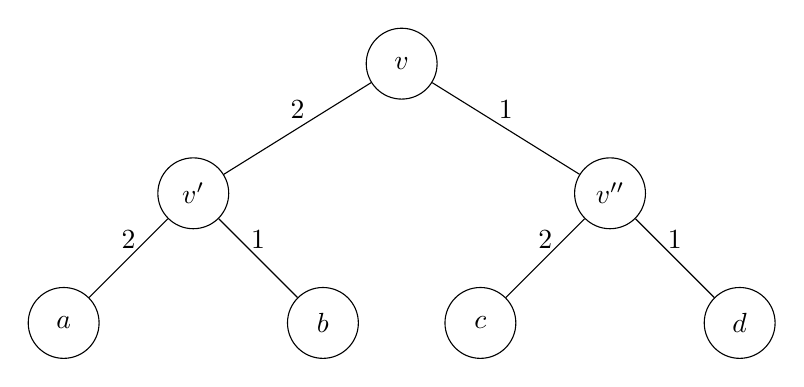
\begin{tikzpicture}
    \node[circle,draw,minimum size=.9cm] (v) {$v$};
    \node[circle,draw,minimum size=.9cm,below left=of v,xshift=-1cm] (vp) {$v'$};
    \node[circle,draw,minimum size=.9cm,below right=of v,xshift=1cm] (vpp) {$v''$};
    \node[circle,draw,minimum size=.9cm,below left=of vp] (a) {$a$};
    \node[circle,draw,minimum size=.9cm,below right=of vp] (b) {$b$};
    \node[circle,draw,minimum size=.9cm,below left=of vpp] (c) {$c$};
    \node[circle,draw,minimum size=.9cm,below right=of vpp] (d) {$d$};
    
    \draw[-] (v) -- (vp) node[above,pos=.5] {2} ;
    \draw[-] (v) -- (vpp) node[above,pos=.5] {1} ;
    \draw[-] (vp) -- (a) node[above,pos=.5] {2};
    \draw[-] (vp) -- (b) node[above,pos=.5] {1};
    \draw[-] (vpp) -- (c) node[above,pos=.5] {2};
    \draw[-] (vpp) -- (d) node[above,pos=.5] {1};
    
  \end{tikzpicture}
  \caption{An instance of the zero-skew problem, described in this problem.  The
    unique optimal solution for this instance would be to take the three
    length-1 edges and increase each of their lengths to 2. The resulting tree
    has zero skew, and the total edge length is 12, the smallest possible.}
\end{figure}

The root generates a clock signal which is propagated along the edges
to the leaves. We’ll assume that the time it takes for the signal to reach a
given leaf is proportional to the distance from the root to the leaf.
Now, if all leaves do not have the same distance from the root, then
the signal will not reach the leaves at the same time, and this is a big
problem. We want the leaves to be completely synchronized, and all to
receive the signal at the same time. To make this happen, we will have to
increase the lengths of certain edges, so that all root-to-leaf paths have
the same length (we’re not able to shrink edge lengths). If we achieve this,
then the tree (with its new edge lengths) will be said to have zero skew.
Our goal is to achieve zero skew in a way that keeps the sum of all the
edge lengths as small as possible.\\


Give an algorithm that increases the lengths of certain edges so that
the resulting tree has zero skew and the \underline{total edge length is as small as
possible}.

Use your algorithm to compute the new edge lengths on
figure~\ref{fig:clock_signal_problem}.

You do not need to prove that your algorithm is correct or prove your
algorithm's runtime, however, you might find it helpful to construct a proof to
double check your work.

\begin{figure}[H]
  \centering
  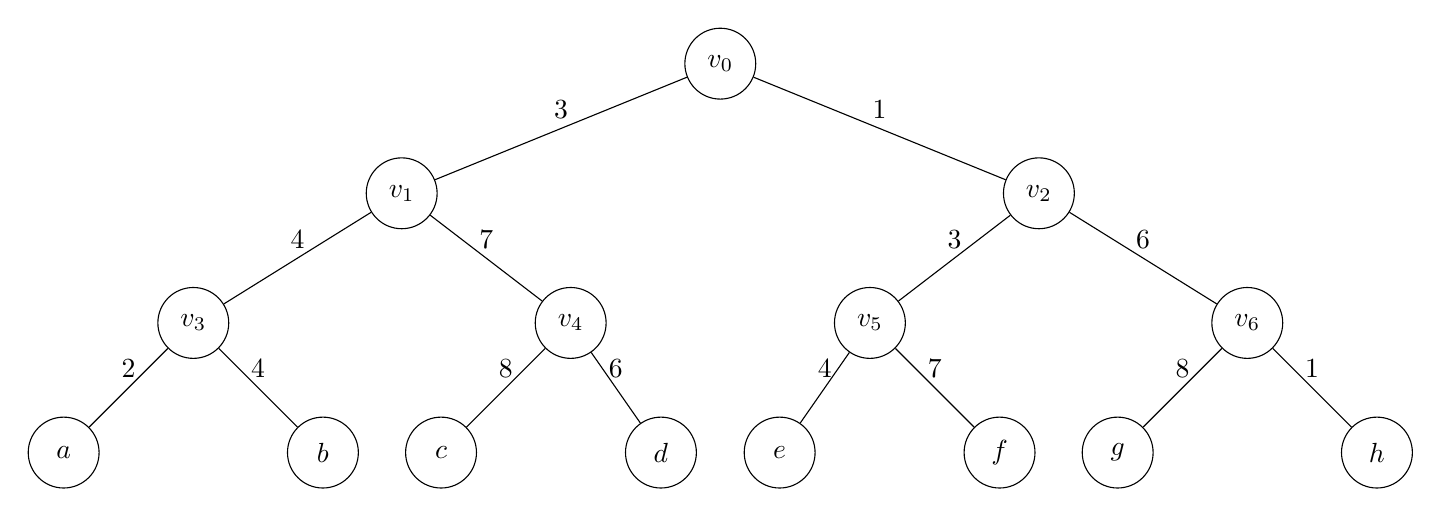
\begin{tikzpicture}[scale=.75]
    \node[circle,draw,minimum size=.9cm] (v) {$v_0$};
    \node[circle,draw,minimum size=.9cm,below left=of v,xshift=-2.4cm] (v1) {$v_1$};
    \node[circle,draw,minimum size=.9cm,below right=of v,xshift=2.4cm] (v2) {$v_2$};
    \node[circle,draw,minimum size=.9cm,below left=of v1,xshift=-1cm] (v3) {$v_3$};
    \node[circle,draw,minimum size=.9cm,below right=of v1,xshift=.5cm] (v4) {$v_4$};
    \node[circle,draw,minimum size=.9cm,below left=of v2,xshift=-.5cm] (v5) {$v_5$};
    \node[circle,draw,minimum size=.9cm,below right=of v2,xshift=1cm] (v6) {$v_6$};
    \node[circle,draw,minimum size=.9cm,below left=of v3] (a) {$a$};
    \node[circle,draw,minimum size=.9cm,below right=of v3] (b) {$b$};
    \node[circle,draw,minimum size=.9cm,below left=of v4] (c) {$c$};
    \node[circle,draw,minimum size=.9cm,below right=of v4,xshift=-.5cm] (d) {$d$};
    \node[circle,draw,minimum size=.9cm,below left=of v5,xshift=.5cm] (e) {$e$};
    \node[circle,draw,minimum size=.9cm,below right=of v5] (f) {$f$};
    \node[circle,draw,minimum size=.9cm,below left=of v6] (g) {$g$};
    \node[circle,draw,minimum size=.9cm,below right=of v6] (h) {$h$};
    
    \draw[-] (v) -- (v1) node[above,pos=.5] {3} ;
    \draw[-] (v) -- (v2) node[above,pos=.5] {1} ;
    \draw[-] (v1) -- (v3) node[above,pos=.5] {4} ;
    \draw[-] (v1) -- (v4) node[above,pos=.5] {7} ;
    \draw[-] (v2) -- (v5) node[above,pos=.5] {3} ;
    \draw[-] (v2) -- (v6) node[above,pos=.5] {6} ;
    \draw[-] (v3) -- (a) node[above,pos=.5] {2} ;
    \draw[-] (v3) -- (b) node[above,pos=.5] {4} ;
    \draw[-] (v4) -- (c) node[above,pos=.5] {8} ;
    \draw[-] (v4) -- (d) node[above,pos=.5] {6} ;
    \draw[-] (v5) -- (e) node[above,pos=.5] {4} ;
    \draw[-] (v5) -- (f) node[above,pos=.5] {7} ;
    \draw[-] (v6) -- (g) node[above,pos=.5] {8} ;
    \draw[-] (v6) -- (h) node[above,pos=.5] {1} ;
  \end{tikzpicture}
  \caption{Show your the new lengths calculated by your algorithm on the above tree.}
  \label{fig:clock_signal_problem}
\end{figure}

\subsection{Solution: Algorithm}

Let the subtrees below the root node $r$ be tree $L$ and tree $R$. \\

If the height (max sum of edge lengths on the path from the parent to the leaf) of $L$ is $x$ more than $R$, where $x > 0$, then we increase the length of edge $(r, R)$ by $x$. \\

If the height (max sum of edge lengths on the path from the parent to the leaf) of $R$ is $x$ more than $L$, where $x > 0$, then we increase the length of edge $(r, L)$ by $x$. \\

Now, we repeat the same process for $L$ and $R$ independently.



\subsection{Solution: Algorithm Performed on Figure}

\begin{figure}[H]
  \centering
  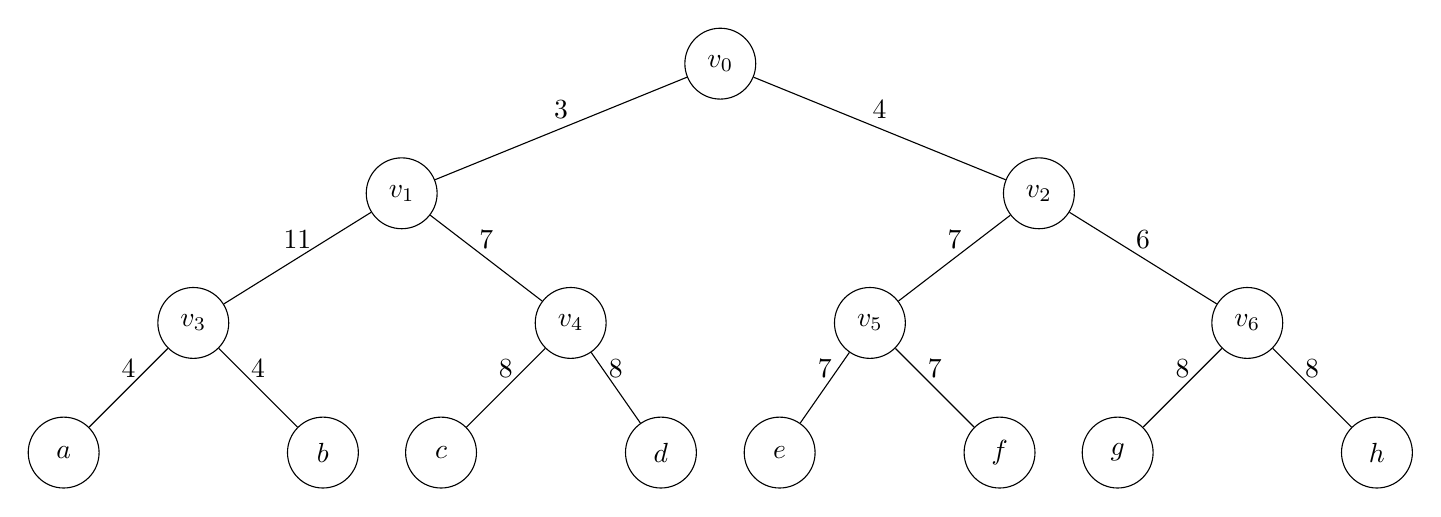
\begin{tikzpicture}[scale=.75]
    \node[circle,draw,minimum size=.9cm] (v) {$v_0$};
    \node[circle,draw,minimum size=.9cm,below left=of v,xshift=-2.4cm] (v1) {$v_1$};
    \node[circle,draw,minimum size=.9cm,below right=of v,xshift=2.4cm] (v2) {$v_2$};
    \node[circle,draw,minimum size=.9cm,below left=of v1,xshift=-1cm] (v3) {$v_3$};
    \node[circle,draw,minimum size=.9cm,below right=of v1,xshift=.5cm] (v4) {$v_4$};
    \node[circle,draw,minimum size=.9cm,below left=of v2,xshift=-.5cm] (v5) {$v_5$};
    \node[circle,draw,minimum size=.9cm,below right=of v2,xshift=1cm] (v6) {$v_6$};
    \node[circle,draw,minimum size=.9cm,below left=of v3] (a) {$a$};
    \node[circle,draw,minimum size=.9cm,below right=of v3] (b) {$b$};
    \node[circle,draw,minimum size=.9cm,below left=of v4] (c) {$c$};
    \node[circle,draw,minimum size=.9cm,below right=of v4,xshift=-.5cm] (d) {$d$};
    \node[circle,draw,minimum size=.9cm,below left=of v5,xshift=.5cm] (e) {$e$};
    \node[circle,draw,minimum size=.9cm,below right=of v5] (f) {$f$};
    \node[circle,draw,minimum size=.9cm,below left=of v6] (g) {$g$};
    \node[circle,draw,minimum size=.9cm,below right=of v6] (h) {$h$};
    
    \draw[-] (v) -- (v1) node[above,pos=.5] {3} ;
    \draw[-] (v) -- (v2) node[above,pos=.5] {4} ;
    \draw[-] (v1) -- (v3) node[above,pos=.5] {11} ;
    \draw[-] (v1) -- (v4) node[above,pos=.5] {7} ;
    \draw[-] (v2) -- (v5) node[above,pos=.5] {7} ;
    \draw[-] (v2) -- (v6) node[above,pos=.5] {6} ;
    \draw[-] (v3) -- (a) node[above,pos=.5] {4} ;
    \draw[-] (v3) -- (b) node[above,pos=.5] {4} ;
    \draw[-] (v4) -- (c) node[above,pos=.5] {8} ;
    \draw[-] (v4) -- (d) node[above,pos=.5] {8} ;
    \draw[-] (v5) -- (e) node[above,pos=.5] {7} ;
    \draw[-] (v5) -- (f) node[above,pos=.5] {7} ;
    \draw[-] (v6) -- (g) node[above,pos=.5] {8} ;
    \draw[-] (v6) -- (h) node[above,pos=.5] {8} ;
  \end{tikzpicture}
  \caption{The new lengths calculated by algorithm, path length 18.}
  \label{fig:clock_signal_solution}
\end{figure}

\section{Graphs Getting Their Degrees (8 points)}

Given a list of $n$ natural numbers $d_1, d_2, \ldots d_n$, give a greedy algorithm that constructs a graph $G$ in polynomial time where the degrees of the nodes are $d_1, d_2, \ldots d_n$.  (That is if $V=\{v_1, v_2, \ldots, v_n\}$, then the degree of $v_i$ should be exactly $d_i$.)  If no such graph $G$ exists, your algorithm should report that it is impossible to construct such a graph.  $G$ should not contain multiple edges between nodes and there are no ``self-loops'' edges in the graph.

\begin{enumerate}
\item Include a description or pseudo code for your algorithm.

\item Include a proof that your algorithm is correct.

\item Use your algorithm to check if there exists a graph $G$ with degrees $L$.  If $G$ exists, include a diagram of $G$ in your homework submission.
\[ L = [ 4, 3, 3, 8, 3, 3, 5, 7, 2, 8, 6 ]. \]
\end{enumerate}

\subsection{Solution: Algorithm}

Let $d_1,...d_n$ be the degree sequence that we want. Let's first sort the degrees in decreasing order, with the largest degree first, and the smallest degree last. \\

If the first degree $d_1$ is negative or greater than $n-1$, where $n$ is the number of nodes, return that the graph cannot be made. \\

Otherwise, remove degree $d_1$ from the list, and decrease the next $d_1$ degrees in the list by 1, while adding the edge in between the nodes that you decreased the degrees from. If there are not enough degrees left in the list to decrease, report that it's impossible to construct such a graph and stop.\\

Repeat the above steps until either we return that the graph cannot be made, or all degrees are reduced to $0$, in which case we have constructed graph $G$. We also resort the degrees in decreasing order every time we remove a degree from the list.\\

If at any point, we cannot proceed because you have a negative degree or not enough degrees left in the list, return that the graph cannot be made.

\subsection{Solution: Proof of Algorithm}

\indent \indent Case One: If all the degrees $d_i = 0$, then the graph exists, because the graph would have $n$ vertices and $0$ edges.

Case Two: All the degrees $d_i \neq 0$. We sort the $d_i$ in decreasing order, with the largest first and the smallest last. Now, we argue that there is a graph with degree sequence $(d_1, d_2, ... d_n)$ if and only if there is a graph with $n-1$ vertices with degree sequence $(d_2-1, d_3-1,...,d_k-1, d_{k+1}, ..., d_n)$, where $k = d_1$. In conclusion, if a graph with sequence $(d_1,...,d_n)$ exists, then we can assume that the highest degree vertex (of degree $d_1$) has edges to the next $d_1$ highest degree vertices.

One direction proof: If there is a graph G with degree sequence $(d_2-1, d_3-1,...,d_k-1,d_{k+1},...,d_n)$ then there is a graph with degree sequence $(d_1,...,d_n)$ as follows: Just add a new certex to G which has edges to the vertices with degrees $d_2-1, d_3-1,...,d_k-1$. 

Proving the reverse: Suppose there is a graph G with degree sequence $(d_1,...,d_n)$. Let $v_i$ be the vertex with degree $d_i$. If $v_i$ has edges to $v_2,...,v_k$ in $G$, then we can just remove $v_1$ and we have the desired graph with the degree sequence we want.

Assume there is an index $i$, $2 \leq i \leq k$ such that $(v_1, v_i)$ is not an edge. Since the degree of $v_1$ is $k (=d_1)$, there must be an index $j > k$ such that $(v_1,v_j)$ is an edge. Since the degree of $v_i$ at least that of $v_j$, there must be a vertex $v_k$ such that $(v_i,v_k)$ is an edge, but $(v_j,v_k)$ is not an edge. In G, we remove the edges $(v_1,v_j)$ and $(v_i,v_k)$ and add the edges $(v_1,v_i)$ and $(v_j,v_k)$. This does not change the degree of any vertex, we have increased the number of edges from $v_1$ to the vertices in the set $\{v_2,...,v_k\}$. Then, we can repeat this process until $v_1$ has edges to $\{v_2,...,v_k\}$.

\subsection{Solution: Created Graph}

Given the below sequence of degrees:

\[ L = [ 4, 3, 3, 8, 3, 3, 5, 7, 2, 8, 6 ]. \]

The following graph is the graph made by the algorithm above.

\[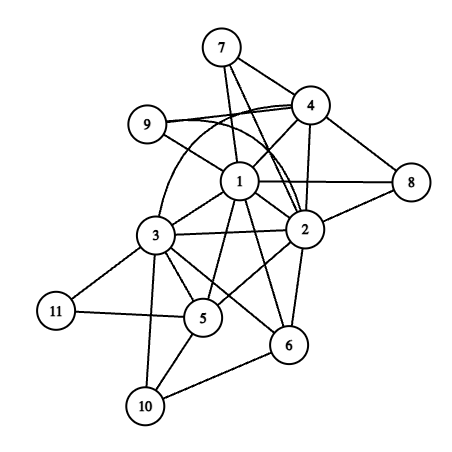
\includegraphics[width=7cm]{graph.png}\]

\section{Only The Max Edge Matters (8 points)}

Let $G = (V, E)$ be an undirected graph with \emph{distinct non-negative} edge weights. Consider a problem similar to the single-source shortest paths problem, but where we define path cost differently. We will define the cost of a simple $s$-$t$ path $P_{s,t} = \{e_1, e_2, \ldots, e_k\}$ to be $$c(P_{s,t}) = \max_{e \in P} w_e$$

The cost of a path is now just the largest weight on that path, rather than the
sum of the weights on the path. Give an algorithm that takes as input an undirected
graph $G = (V, E)$ with \emph{distinct non-negative edge weights}, and a vertex $s \in V$, and
computes the distance from $s$ to every other node in $G$ with the least cost under cost
function $c(\cdot)$. 

Specifically, for each $t \in V$ , find a simple path $$P_{s,t} =
\{(s, v_1), (v_1, v_2), \dots, (v_{k-1}, v_k), (v_k, t)\}$$ connecting $s$ to $t$ such that, letting $S$ denote the set of all simple paths connecting $s$ and $t$, $\text{dist}(s, t) = \min_{P \in S} c(P)$. \\

Provide an algorithm, that runs in $O(|E| \log |V|)$ time, to solve this problem. Prove the correctness of your algorithm using a formal proof technique. Also prove the runtime of you algorithm.

Hint: Can you learn something from the proof provided in the course book.

\subsection{Solution: Algorithm}


Initialize two arrays, $maxWeight[]$ to keep track of the maximum weight on the path from $s$ to each vertex, and $visited[]$ to keep track of which vertices are included in the tree. Initialize maxWeight[s] to 0, and all other maxWeight values to $- \infty$ to ensure they are updated during the algorithm. Also initialize a priority queue vertexQueue to store vertices, using maxWeight as the key. Insert vertex s into the vertexQueue with a key of 0. \\

While the vertexQueue is not empty, do the following: \\

Extract the vertex u with the maximum key (i.e., maximum weight on the path to u) from the vertexQueue. Set visited[u] to true.\\

For each neighboring vertex v of u:\\

If v is not yet visited and the weight of the edge (u, v) is greater than the current maxWeight[v], update maxWeight[v] and insert v into the vertxQueue with the new maxWeight[v] as the key. \\

Once the vertexQueue is empty, the maxWeight array will contain the maximum edge weight from the source vertex to every other vertex in the tree, representing the least cost. \\

\subsection{Solution: Runtime}

The time complexity of this algorithm is $O(|E| \log |V|)$, as the main loop runs in $O(|E|)$ time and each insert and extract operation on the priority queue takes $O(\log|V|)$ time.

\end{document}
